\documentclass[10pt]{article}
\usepackage[T1]{fontenc}
\usepackage[utf8]{inputenc}
\usepackage{microtype}
\usepackage{graphicx}
\usepackage{booktabs}
\usepackage{tabularx}
\usepackage{array}
\usepackage{amsmath,amssymb}
\usepackage{xcolor}
\usepackage{cite}
\usepackage{hyperref}
\usepackage[nameinlink,noabbrev]{cleveref}
\usepackage{placeins}

\definecolor{linkblue}{HTML}{245B8A}
\hypersetup{
  colorlinks=true,
  linkcolor=linkblue,
  citecolor=linkblue,
  urlcolor=linkblue,
  pdfauthor={Adit Patil},
  pdftitle={Bundle Neural Networks for Functional Connectomes}
}

\graphicspath{{generated/figures/}}
\interdisplaylinepenalty=2500
\hyphenation{con-nec-tome con-nec-tomes over-smooth-ing}

\newcommand{\ASD}{autism spectrum disorder}
\newcommand{\ABIDE}{Autism Brain Imaging Data Exchange}
\newcommand{\BuNN}{Bundle Neural Network}
\newcommand{\GCN}{Graph Convolutional Network}
\newcommand{\FC}{functional connectivity}
\newcommand{\BA}{balanced accuracy}
\newcommand{\code}[1]{\texttt{#1}}
% Generated by scripts/build_manuscript_inputs.py; do not edit manually.
\providecommand{\StudyParentRows}{769}
\providecommand{\StudyTechnicalExclusions}{15}
\providecommand{\StudyParticipants}{754}
\providecommand{\StudySites}{18}
\providecommand{\StudyASD}{371}
\providecommand{\StudyControls}{383}
\providecommand{\StudyROIs}{116}
\providecommand{\StudyEdges}{6,670}
\providecommand{\CovariatesBA}{0.5652}
\providecommand{\ConnectomeBA}{0.6401}
\providecommand{\CombinedBA}{0.6336}
\providecommand{\BunnGcnEstimate}{-0.00958}
\providecommand{\BunnGcnCILow}{-0.03665}
\providecommand{\BunnGcnCIHigh}{0.01146}
\providecommand{\BunnGcnP}{0.524}
\providecommand{\PracticalMargin}{0.03}
\providecommand{\BunnElasticEstimate}{-0.05516}
\providecommand{\BunnElasticCILow}{-0.08297}
\providecommand{\BunnElasticCIHigh}{-0.02752}
\providecommand{\BunnElasticP}{0.0018}
\providecommand{\RankEstimate}{-0.00719}
\providecommand{\RankCILow}{-0.01310}
\providecommand{\RankCIHigh}{-0.00105}
\providecommand{\LeaveOneSitePositive}{1}
\providecommand{\SeedPositive}{2}
\providecommand{\FavorableIntervals}{0}
\providecommand{\UnfavorableSeedIntervals}{1}
\providecommand{\GcnParameters}{5,889}
\providecommand{\BunnParameters}{8,529}
\providecommand{\GcnFitHours}{15.09}
\providecommand{\BunnFitHours}{31.14}
\providecommand{\GcnCurveBA}{0.5945}
\providecommand{\BunnCurveBA}{0.5849}


\title{Bundle Neural Networks for Functional Connectomes:\\
Density-Dependent Aggregation and Cross-Site Prediction}
\author{\IEEEauthorblockN{Adit Patil}
\IEEEauthorblockA{School of Scholars\\
Akola, India}}


\begin{document}
\maketitle
\begin{abstract}
Functional connectomes have an obvious graph structure, yet neighborhood
aggregation can harm prediction when every node already contains a global
connectivity profile. We examined whether learned orthogonal bundle transport
changes this density-dependent behavior. The analysis included
\StudyParticipants{} technically eligible ABIDE-I participants from
\StudySites{} sites. A single neural backbone was paired with identity
propagation, a learned-local capacity control, GCN aggregation, trivial-bundle
diffusion, or learned BuNN transport at positive edge densities of 0, 1, 5, 10,
and 20 percent. We used nested held-out-site validation, five final seeds,
regularized non-graph baselines, and representation diagnostics computed in a
common frame. The primary BuNN-minus-GCN performance-curve contrast was
\BunnGcnEstimate{} (95\% site-bootstrap CI [\BunnGcnCILow{},
\BunnGcnCIHigh{}]; exact sign-flip $p=\BunnGcnP$). Relative to the connectome
elastic net, the BuNN contrast was \BunnElasticEstimate{} (95\% CI
[\BunnElasticCILow{}, \BunnElasticCIHigh{}]). The matched-anchor
effective-rank contrast was \RankEstimate{} (95\% CI [\RankCILow{},
\RankCIHigh{}]), which ran counter to the proposed preservation advantage.
Site weighting and training seed affected the small BuNN-GCN difference. For
this ABIDE-I pipeline, learned bundle transport provided no detected
predictive or representation-preservation advantage. This finding concerns a
computational operator under a specified analysis; it does not establish a
biological bundle geometry or a general result for BuNNs.
\end{abstract}

\section{Introduction}

Resting-state functional connectomes summarize statistical associations among
regional blood-oxygen-level-dependent time series. Representing brain regions
as nodes and functional associations as edges makes graph learning an
intuitive modeling choice. Yet the common node feature in connectome studies
is itself an entire row of the connectivity matrix, so each node begins with a
global connectivity profile rather than purely local information. In this
setting, neighborhood aggregation may remove useful distinctions instead of
adding missing context.

Recent multi-dataset benchmarking reported that classical models and
non-graph neural networks can match or exceed graph deep-learning models for
functional-connectome prediction, and isolated message aggregation as a
potential source of degradation \citep{han2026rethinking}. That result changes
the relevant question. The value of a graph operator should not be presumed
from the fact that the input can be drawn as a graph; it should be demonstrated
against identity propagation and strong regularized baselines under the same
data splits.

BuNNs diffuse features after transporting them through learned orthogonal maps
between node-specific frames \citep{bamberger2025bundle}. Their theoretical and
synthetic motivation includes greater control over representation collapse
than ordinary graph diffusion. Related neural-sheaf work likewise shows that
non-trivial transport can change diffusion behavior \citep{bodnar2022sheaf}.
Whether that advantage transfers to dense functional connectomes with global
connectivity-profile features is an empirical question.

The initial formulation of this project connected negative functional
correlations with heterophilic message passing. Formalizing the experiment
showed that this interpretation was not identifiable: correlation sign does
not establish node-label heterophily, excitation, inhibition, anatomical
connectivity, or causal information flow, and sign can depend on preprocessing
choices such as global-signal regression \citep{murphy2017global}. The dataset,
BuNN architecture, connectome representation, and aggregation problem were
therefore retained, while the hypothesis was narrowed to a controlled operator
comparison.

This study asks whether learned bundle transport produces a more favorable
held-out-site performance-density curve than GCN aggregation, whether any
advantage exceeds identity and learned-local controls as well as a regularized
connectome baseline, and whether predictive behavior co-occurs with
common-frame representation preservation. The contribution is an audit of an
architectural inductive bias under one pre-specified ABIDE-I pipeline, not a
claim about biological geometry or clinical diagnosis.

\section{Related work}

\paragraph{Functional-connectome prediction.}
ABIDE-I aggregated resting-state fMRI and phenotypic data across international
sites to support large-scale autism research \citep{dimartino2014abide}. The
Preprocessed Connectomes Project subsequently released derivatives from
several pipelines, including C-PAC \citep{abidepcp}. Multi-site prediction is
challenging because acquisition, motion, demographics, and preprocessing can
vary across sites. Held-out-site evaluation therefore addresses a stricter
generalization problem than random participant splitting.

\paragraph{Graph aggregation.}
GCNs apply normalized neighborhood aggregation followed by learned feature
transformation \citep{kipf2017gcn}. Repeated diffusion can contract node
representations, although the practical effect depends on architecture,
features, graph construction, and task. In functional connectomes, the problem
is especially relevant because connectivity-row node features already contain
whole-graph information. The benchmark of \citet{han2026rethinking} motivates
testing propagation against a no-propagation control rather than comparing
only different GNN families.

\paragraph{Learned transport.}
Neural sheaf diffusion assigns vector spaces and learned maps to graph
incidences, allowing non-trivial transport before aggregation
\citep{bodnar2022sheaf}. BuNN specializes this idea to flat vector bundles with
orthogonal node maps and diffusion-based propagation
\citep{bamberger2025bundle}. Raw embeddings from different node frames cannot
be compared naively; meaningful collapse diagnostics require transport to a
common frame or a gauge-invariant measure. The present experiment therefore
separates raw map-generator capacity from inter-node transport using a
learned-local control.

\section{Methods}

% Claims C01, C02, C03, C04, C05, C06, C09, C10
\subsection{Study design}

\begin{figure}[t]
  \centering
  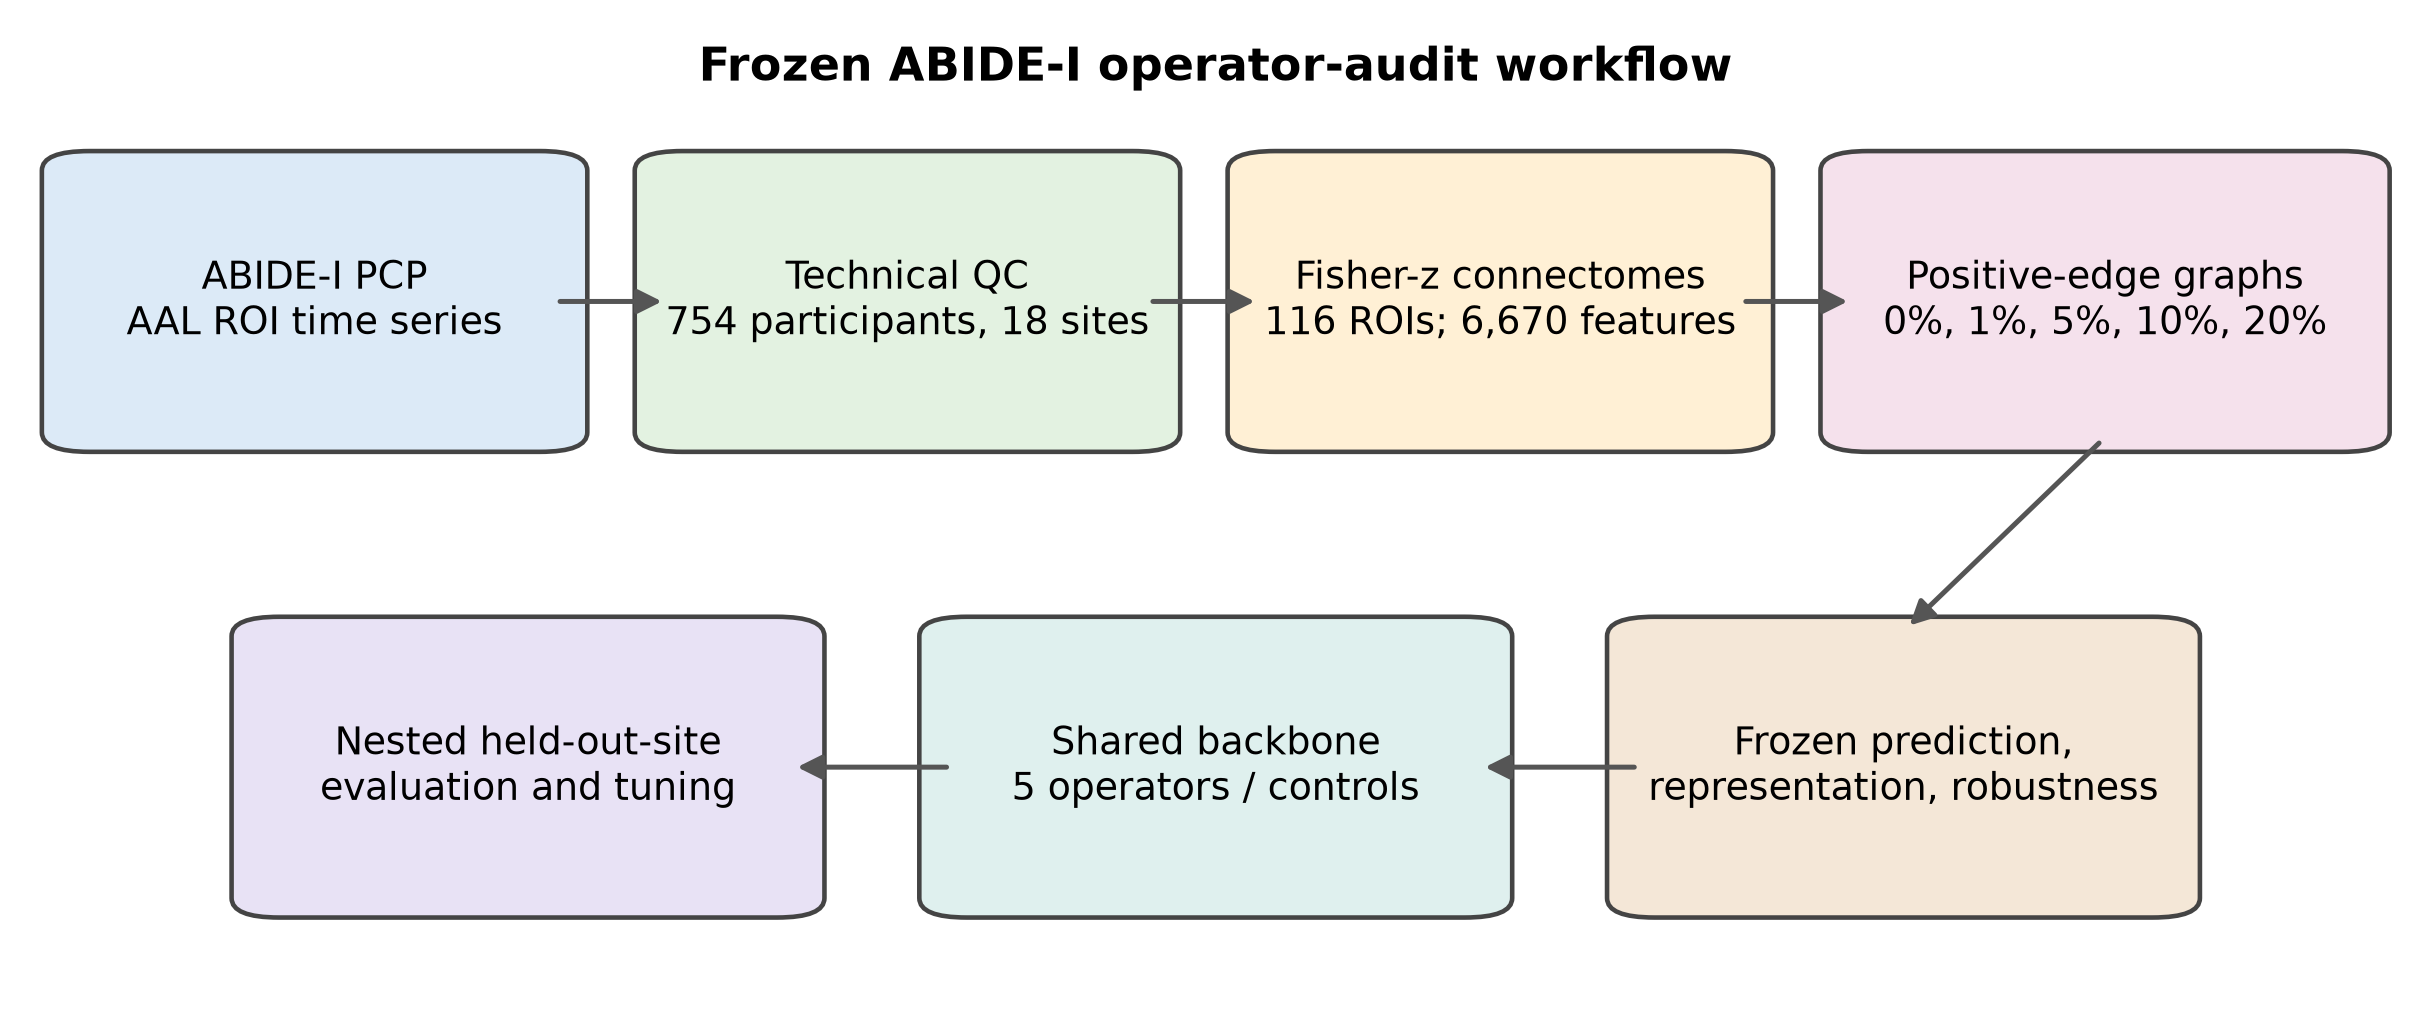
\includegraphics[width=\textwidth]{study_design.png}
  \caption{Frozen study workflow. All feature preprocessing, model selection,
  and hyperparameter selection were confined to training sites. The final
  held-out site was used only for evaluation.}
  \label{fig:study-design}
\end{figure}

The protocol was organized as a controlled operator audit
(\cref{fig:study-design}). Classical baselines were completed and independently
audited first. A shared neural backbone was then paired with five propagation
or capacity-control variants. All neural configurations used the same outer
sites, inner grouped folds, candidate budget, stopping rule, and final seeds.
The complete neural artifact was audited without revealing performance values;
confirmatory analysis code and decision rules were frozen before unblinding.

\subsection{Dataset and technical quality control}

We used ABIDE-I C-PAC derivatives distributed by the Preprocessed Connectomes
Project \citep{dimartino2014abide,abidepcp}. The frozen source was the
band-pass-filtered, no-global-signal-regression AAL ROI time-series derivative.
The AAL atlas defines macroscopic anatomical regions in standardized space
\citep{tzourio2002aal}. A downloaded file was technically eligible only if it
had a valid header, finite numeric values, non-zero variance for every ROI, and
produced a finite connectome. Of \StudyParentRows{} downloaded files,
\StudyTechnicalExclusions{} failed the zero-variance requirement, leaving
\StudyParticipants{} participants (\StudyASD{} ASD and \StudyControls{}
controls) across \StudySites{} evaluable sites. These rules establish technical
eligibility, not population representativeness.

\begin{table}[!t]
\centering
\caption{Cohort retained after technical quality control and resulting connectome dimensions.}
\label{tab:cohort}
\footnotesize
\begin{tabular}{lr}
\toprule
Item & Value \\
\midrule
Downloaded AAL time-series files & 769 \\
Technical exclusions & 15 \\
Retained participants & 754 \\
ASD / control & 371 / 383 \\
Held-out sites & 18 \\
ROIs / lower-triangle features & 116 / 6,670 \\
\bottomrule
\end{tabular}
\end{table}


\subsection{Connectomes, node features, and graphs}

For each participant, Pearson correlations were computed between all pairs of
\StudyROIs{} ROI time series and transformed with Fisher's $r$-to-$z$
transformation. Diagonal entries were set to zero. The resulting matrix was
finite and symmetric, and its \StudyEdges{} lower-triangle values formed the
classical feature vector. Each neural node received its full connectivity row
as a \StudyROIs{}-dimensional feature, so node inputs were globally informed.

For nonzero graph conditions, the strongest positive off-diagonal associations
were retained symmetrically at densities of 1, 5, 10, and 20 percent. Density
zero contained only the matched identity or learned-local anchor. Negative
associations were excluded as a pre-specified computational choice and were
not interpreted biologically.

\subsection{Classical baselines}

Three logistic baselines were fit: covariates only, vectorized connectomes with
elastic-net regularization, and connectomes plus covariates. Elastic-net
regularization combines $\ell_1$ and $\ell_2$ penalties and is appropriate for
correlated high-dimensional predictors \citep{zou2005elastic}. Covariates were
age, sex, mean framewise displacement, and usable scan length. Scaling,
feature processing, and tuning were fit using training sites only.

\subsection{Shared neural backbone and operators}

The encoder, hidden width, depth, nonlinearities, normalization, dropout,
pooling, classifier, optimizer, training schedule, and tuning budget were held
constant. The variants were:

\begin{enumerate}
  \item \textbf{Identity}: no inter-node propagation.
  \item \textbf{Learned-local}: the BuNN map generator and node-wise updates,
  but no inter-node diffusion, controlling for additional learned capacity.
  \item \textbf{GCN}: normalized neighborhood aggregation
  \citep{kipf2017gcn}.
  \item \textbf{Trivial bundle}: the same diffusion construction with identity
  transport maps.
  \item \textbf{Learned BuNN}: learned orthogonal node maps followed by bundle
  diffusion \citep{bamberger2025bundle}.
\end{enumerate}

\subsection{Nested held-out-site evaluation}

Each of the \StudySites{} sites served once as the outer test site. Within the
remaining sites, four grouped inner folds selected among four equal-budget
AdamW candidates using two tuning seeds. The selected configuration was refit
with five fixed final seeds. Predictions from a test site were never used for
scaling, tuning, early stopping, or configuration selection. The primary
predictive endpoint was equal-site mean balanced accuracy; pooled balanced
accuracy and AUROC were secondary summaries.

\subsection{Density curves and representation diagnostics}

The primary predictive estimand was the normalized trapezoidal area under the
balanced-accuracy curve across the complete density grid. GCN and
trivial-bundle curves used identity at density zero; the learned-BuNN curve used
the parameter-matched learned-local anchor. This prevented a favorable density
from replacing the pre-specified curve-level comparison.

After each propagation layer, embeddings were mapped to a common learned frame
before cross-node comparison. The primary representation endpoint was
normalized effective rank at layer 2. Normalized dispersion, mean pairwise
cosine similarity, invariant edge-transport distance, and encoder-to-layer-2
rank change were secondary. Predictive and representation behavior were tested
as co-occurring outcomes; no mediation or causal claim was made.

\subsection{Statistical analysis and decision rule}

Five final seeds were averaged within each site and configuration before
site-level inference. Paired percentile intervals used 10,000 bootstrap
resamples of the \StudySites{} held-out sites. Exact two-sided paired sign-flip
tests accompanied curve contrasts. Density-specific tests were secondary and
Holm-corrected within each named contrast family.

A complete positive BuNN result required all three pre-specified conditions:
better representation preservation than GCN, better held-out prediction than
GCN and no-propagation controls, and performance exceeding the strongest
regularized baseline. A confidence interval containing zero was reported as no
advantage detected. Absence of a practically meaningful gain was asserted only
when the upper bound excluded the pre-specified +\PracticalMargin{} balanced-
accuracy margin.

\subsection{Run integrity and reproducibility}

Long runs used atomic per-site checkpoints, immutable data/configuration/source
hashes, deterministic site ownership, resume validation, and independent
completion audits. The accepted neural run contained all outer sites and
passed the frozen coverage, recomputation, diagnostic, runtime, and warning
checks before the result embargo was lifted. Paper values are generated from a
hash-bound result snapshot rather than typed independently.

\section{Results}

% Claims C01 and C02
\subsection{Cohort and classical baselines}

After technical quality control, \StudyParticipants{} participants remained
across \StudySites{} held-out sites (\cref{tab:cohort}). The connectome elastic
net had the highest equal-site balanced accuracy among the classical models
(\ConnectomeBA{}). The corresponding values were \CombinedBA{} for connectomes
plus covariates and \CovariatesBA{} for covariates alone
(\cref{tab:baselines}). These cross-site results describe computational
prediction, not clinical diagnostic performance.

\begin{table}[t]
\centering
\caption{Classical held-out-site baselines. Equal-site balanced accuracy is the primary summary.}
\label{tab:baselines}
\begin{tabular}{lccc}
\toprule
Model & Equal-site BA & Pooled BA & Pooled AUROC \\
\midrule
Covariates-only logistic regression & 0.5652 & 0.5629 & 0.5973 \\
Connectome elastic net & 0.6401 & 0.6495 & 0.6794 \\
Connectome + covariates elastic net & 0.6336 & 0.6428 & 0.6773 \\
\bottomrule
\end{tabular}
\end{table}


% Claims C03, C04, C05 and C10
\subsection{Predictive density curves}

\begin{figure}[H]
  \centering
  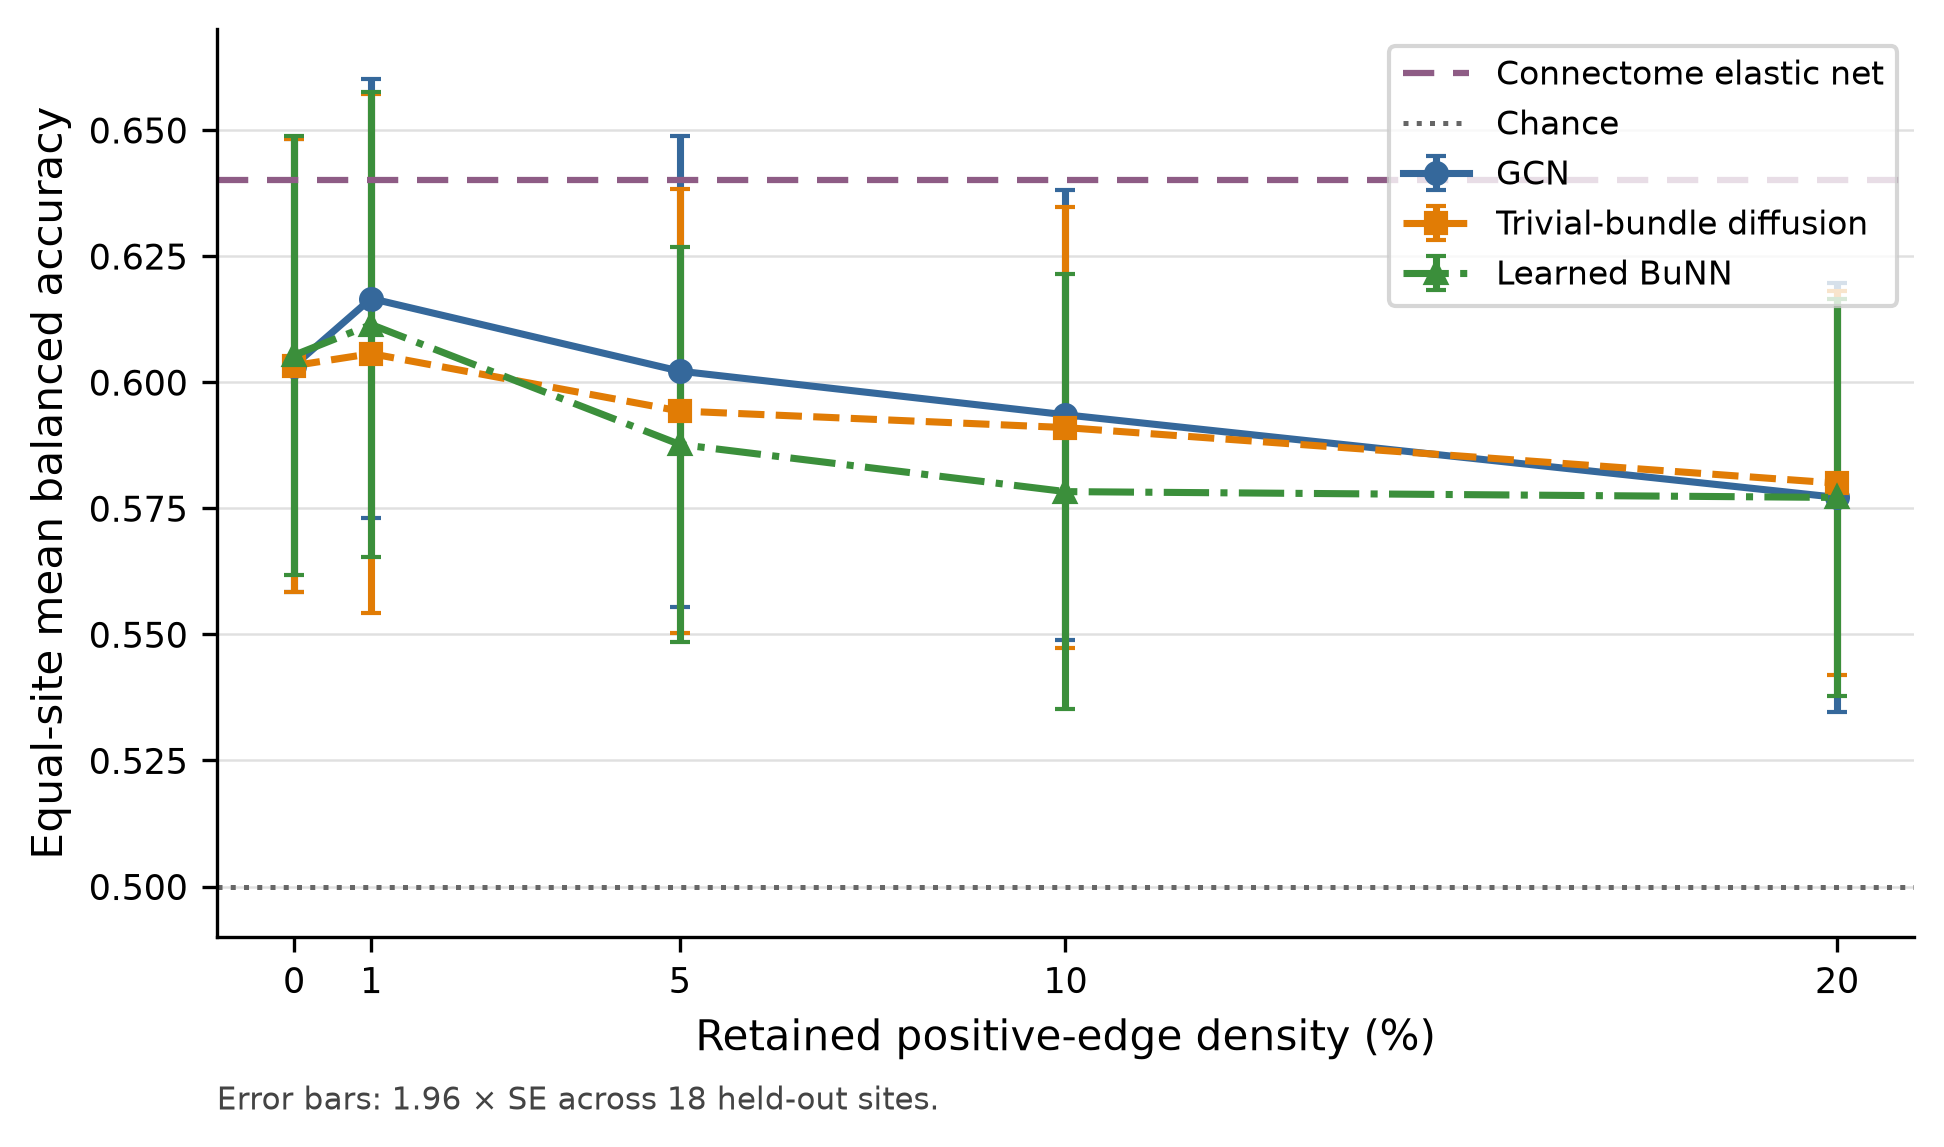
\includegraphics[width=0.98\textwidth]{predictive_density_curves.png}
  \caption{Equal-site mean held-out balanced accuracy across the pre-specified
  positive-edge density grid. Error bars show 1.96 standard errors across sites
  for visualization; confirmatory inference used paired site bootstrap and
  exact sign-flip tests on the locked curve estimand.}
  \label{fig:predictive-curves}
\end{figure}

All three diffusion curves declined as density increased
(\cref{fig:predictive-curves}). The normalized curve-area difference for
learned BuNN minus GCN was \BunnGcnEstimate{} (95\% site-bootstrap CI
[\BunnGcnCILow{}, \BunnGcnCIHigh{}]; exact $p=\BunnGcnP$). Because the interval
crossed zero, we detected no predictive advantage. The upper bound also fell
below the pre-specified +\PracticalMargin{} margin. This rules out a gain of
that size for the chosen estimand and pipeline, but it neither establishes
universal equivalence nor excludes smaller gains.

Against the site-matched connectome elastic net, the learned-BuNN curve
difference was \BunnElasticEstimate{} (95\% CI [\BunnElasticCILow{},
\BunnElasticCIHigh{}]; exact $p=\BunnElasticP$). Comparisons with identity
propagation and the learned-local control also failed the positive-result rule
(\cref{tab:confirmatory}).

\begin{table*}[!t]
\centering
\caption{Pre-specified predictive contrasts. Differences are BuNN minus the named comparator.}
\label{tab:confirmatory}
\footnotesize
\begin{tabularx}{\textwidth}{Xrrr}
\toprule
Contrast & Estimate & 95\% site-bootstrap CI & Exact $p$ \\
\midrule
BuNN curve - GCN curve & -0.0096 & [-0.0366, 0.0115] & 0.5237 \\
BuNN curve - trivial-bundle curve & -0.0062 & [-0.0293, 0.0108] & 0.6813 \\
BuNN nonzero mean - learned-local & -0.0167 & [-0.0347, 0.0009] & 0.0958 \\
BuNN nonzero mean - identity & -0.0146 & [-0.0320, 0.0018] & 0.1155 \\
BuNN curve - connectome elastic net & -0.0552 & [-0.0830, -0.0275] & 0.0018 \\
\bottomrule
\end{tabularx}
\end{table*}


% Claim C06
\subsection{Common-frame representation diagnostics}

\begin{figure}[H]
  \centering
  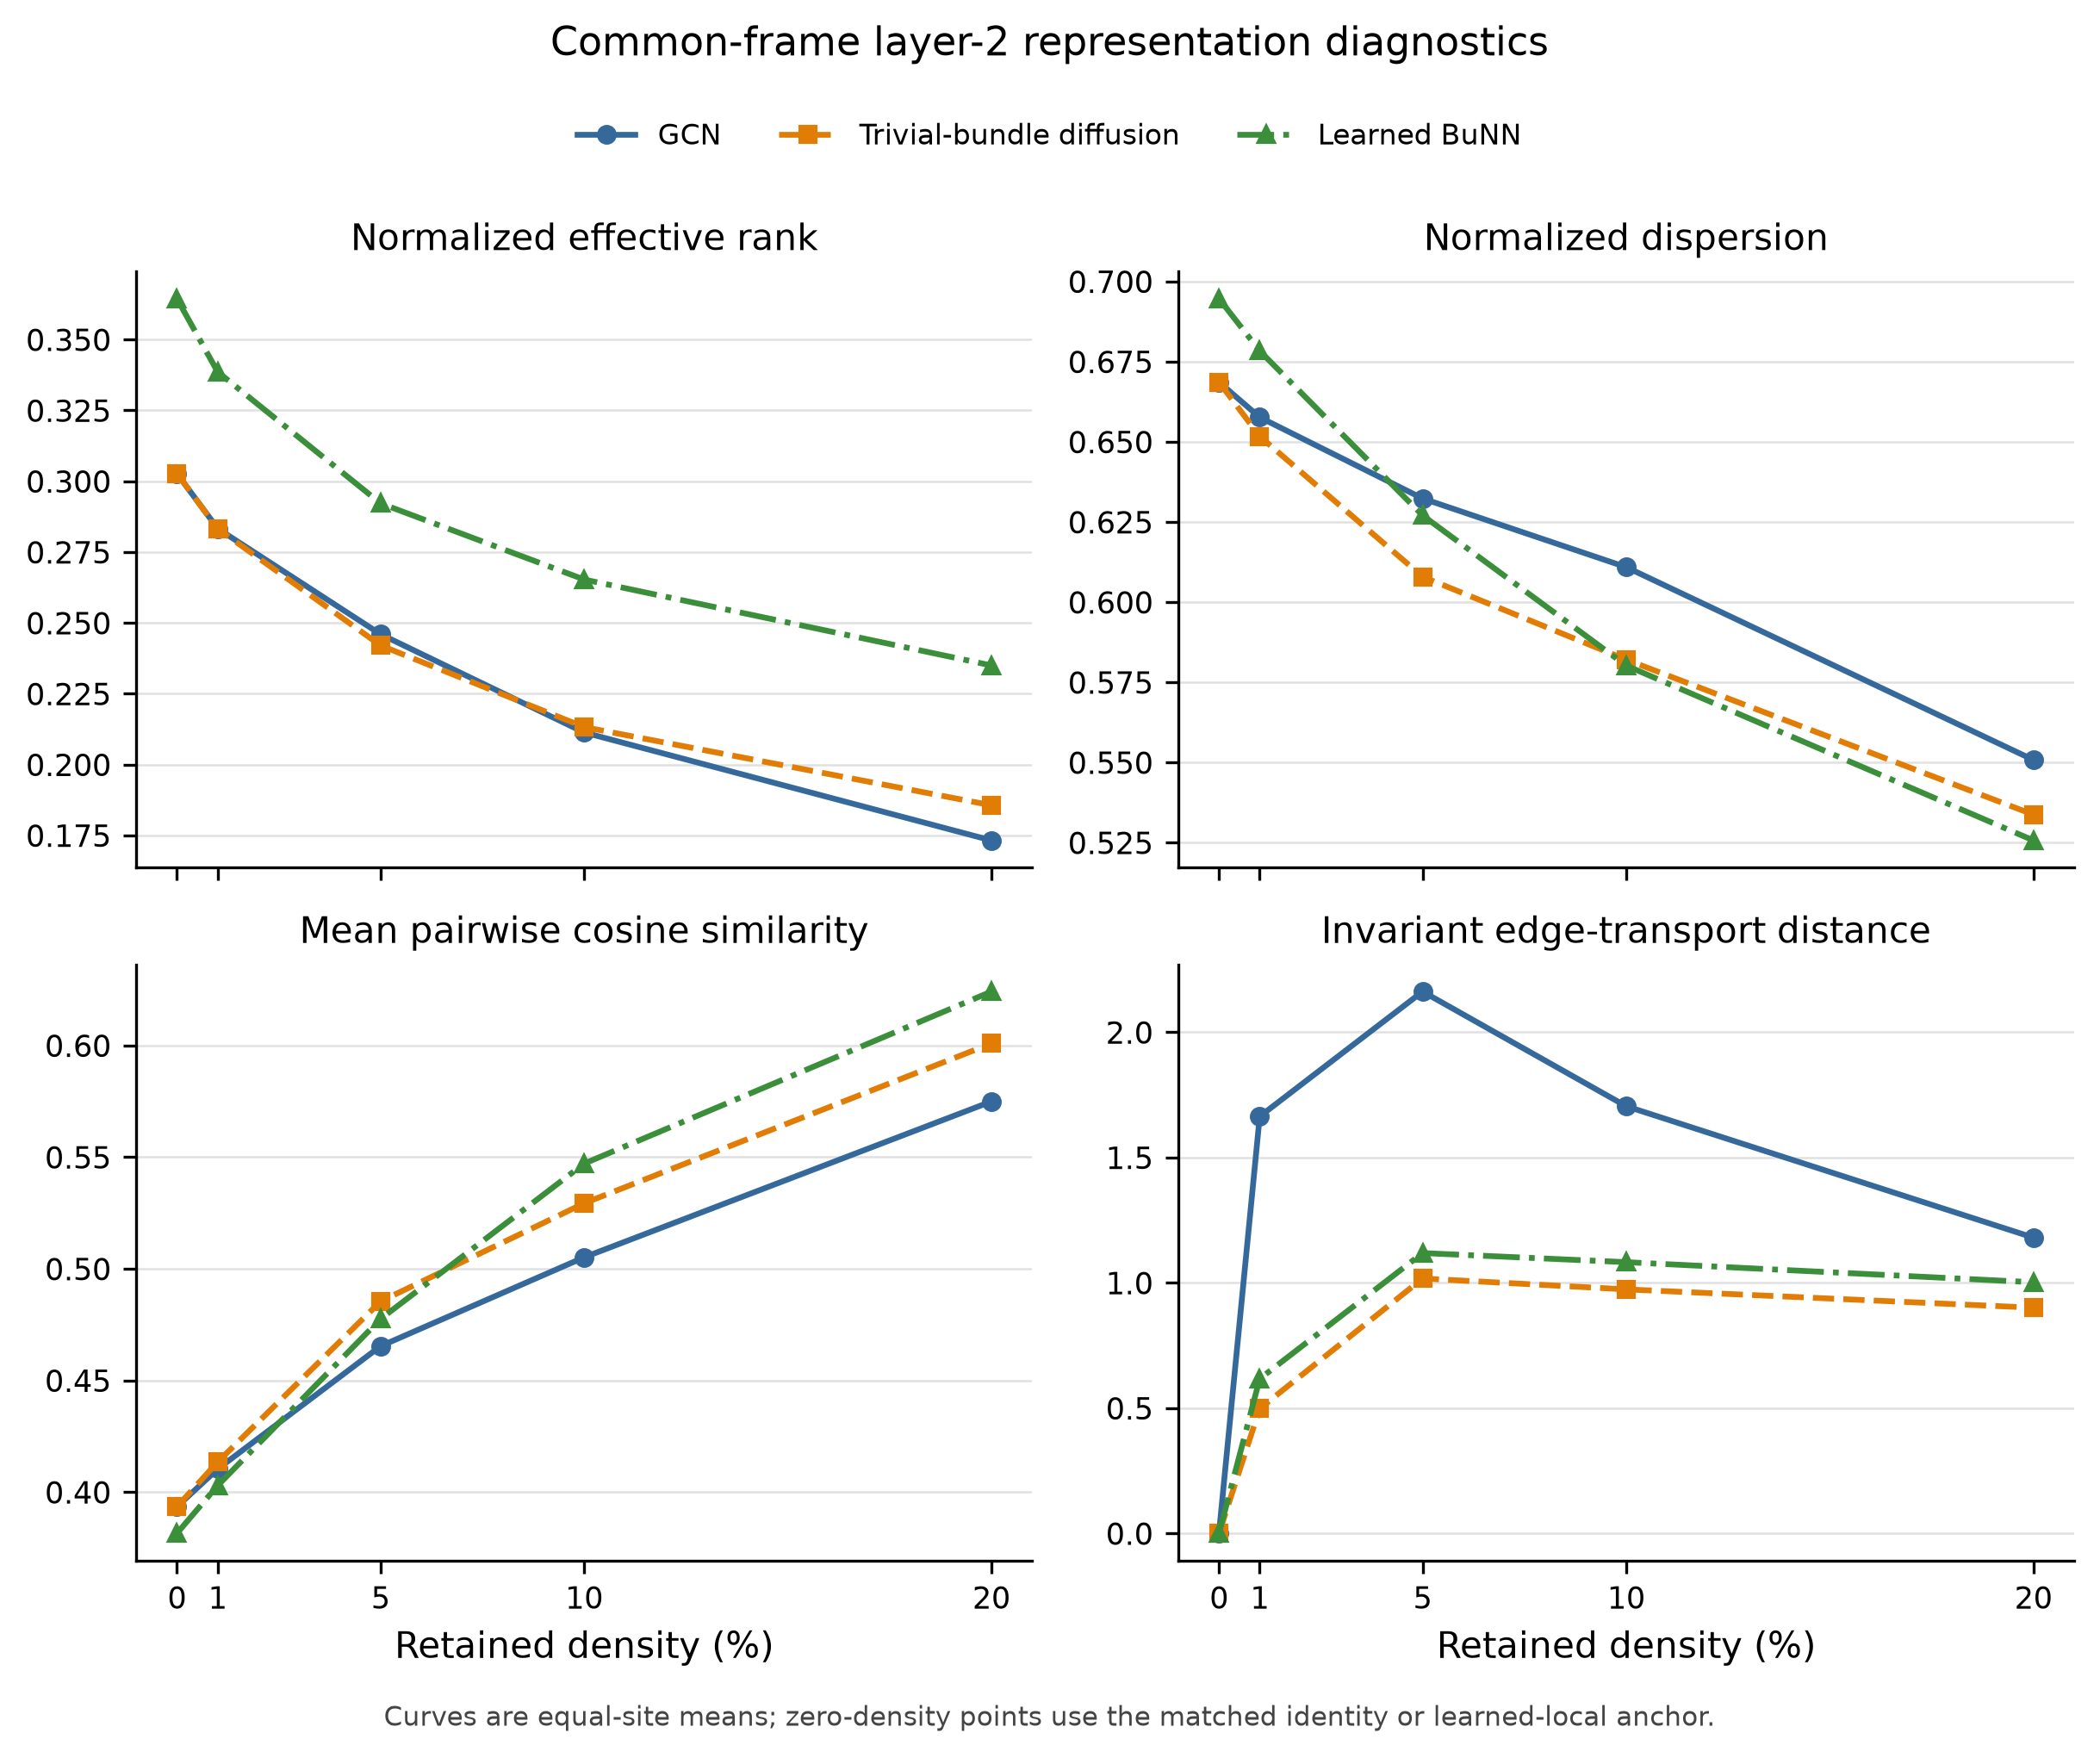
\includegraphics[width=\textwidth]{representation_density_curves.png}
  \caption{Equal-site means for common-frame layer-2 representation
  diagnostics. Zero-density points use the matched identity or learned-local
  anchor. Raw unaligned BuNN node embeddings were not compared.}
  \label{fig:representation}
\end{figure}

The matched-anchor normalized effective-rank contrast was \RankEstimate{}
(95\% CI [\RankCILow{}, \RankCIHigh{}]), the opposite of the proposed BuNN
preservation advantage. Although the raw BuNN rank curve was higher, its
learned-local anchor already included the extra map-generator capacity. The
matched contrast did not support attributing the raw difference to inter-node
bundle transport. Dispersion and cosine similarity pointed in the same
direction (\cref{fig:representation}). None of these diagnostics identifies a
biological mechanism.

% Claims C07 and C08
\subsection{Site, seed, and weighting sensitivity}

Only \LeaveOneSitePositive{} of the \StudySites{} leave-one-site estimates was
positive, and no favorable exclusion interval lay above zero (Supplementary
Figure S1). Of the five final seeds, \SeedPositive{} point estimates favored
BuNN, but \FavorableIntervals{} favorable intervals excluded zero.
\UnfavorableSeedIntervals{} unfavorable seed interval lay below zero
(Supplementary Figure S2). Participant weighting reversed the sign of the
small BuNN-GCN point estimate; the equal-site mean and median remained
negative. The pre-specified confirmatory estimand used equal-site weighting.

% Claim C09
\subsection{Observed execution cost}

Learned BuNN used \BunnParameters{} parameters, compared with \GcnParameters{}
for GCN. Its recorded fits required \BunnFitHours{} total fit-hours, while GCN
required \GcnFitHours{}. Equal-site curve balanced accuracy was lower for BuNN
(\BunnCurveBA{} versus \GcnCurveBA{}). The timings apply to this implementation
on an A10G GPU and should not be read as universal complexity estimates.

\begin{table}[H]
\centering
\caption{Observed execution cost and predictive curve summary for the three diffusion operators. Runtime is implementation- and hardware-specific.}
\label{tab:efficiency}
\small
\begin{tabular}{lrrrrr}
\toprule
Operator & Params. & Fit h & s/fit & Peak GiB & Curve BA \\
\midrule
GCN & 5,889 & 15.09 & 20.39 & 0.373 & 0.5945 \\
Trivial-bundle diffusion & 5,889 & 25.99 & 35.12 & 0.377 & 0.5911 \\
Learned BuNN & 8,529 & 31.14 & 42.08 & 0.378 & 0.5849 \\
\bottomrule
\end{tabular}
\end{table}


\section{Discussion}

% Claims C03-C10
This controlled audit found no complete transfer of the proposed BuNN
anti-collapse advantage to the specified ABIDE-I functional-connectome
pipeline. Learned bundle transport did not improve the primary performance-
density curve relative to GCN, did not exceed the strongest regularized
connectome baseline, and did not show the proposed matched-anchor effective-
rank advantage. The result is scientifically useful because the design
isolated propagation from backbone, input, tuning-budget, and capacity
differences.

\subsection{Why transport may not help in this setting}

Two properties distinguish this task from the settings that motivate bundle
transport. First, functional-connectome graphs are dense even after thresholding.
Second, the feature attached to each node is its full connectivity row, so each
node already contains global information before propagation. Diffusion may
therefore average globally informative profiles rather than deliver missing
long-range context. The downward descriptive density curves are consistent
with density-dependent aggregation degradation, but do not alone prove a
general over-smoothing mechanism.

\subsection{Importance of the learned-local control}

BuNN contains additional learned map-generator parameters. A comparison with
GCN alone could confuse transport with added node-wise capacity. The
learned-local control retained this capacity while removing inter-node
diffusion. Its high raw effective rank showed why unaligned or unmatched rank
curves could falsely appear to support bundle transport. The matched-anchor
analysis instead tested what changed when inter-node transport was added.

\subsection{Heterogeneity and uncertainty}

The primary BuNN-GCN interval crossed zero, and its point estimate changed sign
under participant weighting. Site exclusions and final seeds also changed the
magnitude and sometimes the direction of the small contrast. These analyses do
not reveal a hidden positive result; they show that a small average effect is
unstable relative to multi-site and optimization variation. In contrast, the
negative BuNN-versus-elastic-net result and matched-anchor effective-rank
finding were stable across all leave-one-site exclusions.

\subsection{Limitations}

The conclusions are conditional on ABIDE-I, C-PAC filtered data without global-
signal regression, the AAL-116 atlas, Pearson/Fisher-$z$ connectomes, positive-
edge thresholding, connectivity-profile node features, the fixed density grid,
the shared backbone, and the equal tuning budget. Functional correlations do
not identify anatomy or causal information flow. The study has no locked
external validation cohort, and site sample sizes vary substantially. Runtime
comparisons depend on this implementation and hardware. Finally, the
representation diagnostics measure computational behavior; they do not show
that a representation change caused a predictive change.

\subsection{Future work}

The next scientifically clean extension would freeze the complete ABIDE-I code
and evaluate it on a preprocessing-compatible ABIDE-II cohort. Separate
pre-registered sensitivity studies could test global-signal regression,
negative-edge handling, another atlas, or node features that do not already
encode the full connectome. Such studies should remain distinct from the
present confirmatory result and should not search across datasets for a
favorable diagnosis.

\section{Conclusion}

In this pre-specified ABIDE-I pipeline, learned orthogonal bundle transport did
not improve the held-out-site performance-density curve over GCN. It also
failed to surpass identity propagation or the learned-local control and
remained below the regularized connectome baseline. Gauge-aware,
matched-anchor diagnostics offered no evidence for the proposed
representation-preservation advantage. Bundle transport changed the operator
and increased both model capacity and runtime, but we detected no predictive
benefit in this dense connectome setting with globally informed node features.


\section*{Data and code availability}
The analysis uses the public ABIDE-I Preprocessed Connectomes Project
derivatives. The reproducibility package records the exact data manifest,
technical exclusions, site splits, configurations, seeds, source hashes,
analysis scripts, and aggregate result artifacts. Participant-linked audit
artifacts remain separated from the public-safe release package.

\section*{Acknowledgements}
The author thanks the investigators who shared data through ABIDE and the
Preprocessed Connectomes Project. Computational experiments were performed on
an NVIDIA A10G cloud instance. AI-assisted tools were used for literature
retrieval, code review, debugging, and document preparation; their use is
recorded in the version-controlled provenance log.

\bibliographystyle{plainnat}
\bibliography{references}
\end{document}
